\section{障碍问题}
\label{sec:nlipm-barrier}

约束是一般的光滑函数时，怎样把“不许越界”写进目标，又让解最终能落到边界上？做法是求解一族带参数的内点子问题，再逐步减小参数。

\paragraph{问题与贯穿例}
本章讨论光滑约束问题
\begin{equation}
 \min_{\bm{x}\in\mathbb{R}^n}\ f(\bm{x})\quad\text{s.t.}\quad g_i(\bm{x})\leq0\ (i=1,\ldots,m),\quad h_j(\bm{x})=0\ (j=1,\ldots,p),
 \label{eq:nlipm-problem}
\end{equation}
其中$f$、$g_i$、$h_j$二阶连续可微。把约束值排成向量$\bm{g}(\bm{x})$、$\bm{h}(\bm{x})$，把它们的梯度按行排成两个Jacobian矩阵：
\begin{equation}
 \bm{J}(\bm{x})=\begin{bmatrix}\nabla g_1(\bm{x})^\top\\\vdots\\\nabla g_m(\bm{x})^\top\end{bmatrix}\in\mathbb{R}^{m\times n},\qquad
 \bm{A}(\bm{x})=\begin{bmatrix}\nabla h_1(\bm{x})^\top\\\vdots\\\nabla h_p(\bm{x})^\top\end{bmatrix}\in\mathbb{R}^{p\times n}.
 \label{eq:nlipm-jacobians}
\end{equation}
本章的$\bm{g}$始终表示约束值，不表示目标的梯度；目标梯度写成$\nabla f$。

全章贯穿下面这个二维例子：
\begin{equation}
 \begin{aligned}
 \min_{\bm{x}}\quad&f(\bm{x})=\tfrac12\bigl((x_1-3)^2+x_2^2\bigr)\\
 \text{s.t.}\quad&g_1(\bm{x})=x_1^2-x_2\leq0,\\
 &g_2(\bm{x})=x_2-4\leq0.
 \end{aligned}
 \label{eq:nlipm-running}
\end{equation}
可行集是抛物线之上、直线$x_2=4$之下的区域，目标是到点$\bm{c}=(3,0)^\top$的距离平方的一半。$g_1$是弯的约束，$g_2$是线性约束。

第~\ref{chap:constrained-optimality}章的KKT条件用到Lagrange函数
\begin{equation}
 \mathcal{L}(\bm{x},\bm{\lambda},\bm{\nu})=f(\bm{x})+\bm{\lambda}^\top\bm{g}(\bm{x})+\bm{\nu}^\top\bm{h}(\bm{x}).
 \label{eq:nlipm-lagrangian}
\end{equation}
条件是说：可行点$\bm{x}^\star$处存在乘子$\bm{\lambda}^\star\geq\bm{0}$和$\bm{\nu}^\star$，使$\mathcal{L}$对$\bm{x}$的梯度为零，并且$\lambda_i^\star g_i(\bm{x}^\star)=0$。

例~\eqref{eq:nlipm-running}中取$\bm{x}^\star=(1,1)^\top$，这时两个约束值和三个梯度是
\[
 g_1=0,\quad g_2=-3,\quad\nabla f=\begin{bmatrix}-2\\1\end{bmatrix},\quad\nabla g_1=\begin{bmatrix}2\\-1\end{bmatrix},\quad\nabla g_2=\begin{bmatrix}0\\1\end{bmatrix}.
\]
于是$\bm{\lambda}^\star=(1,0)^\top$满足全部KKT条件，最优值$f^\star=5/2$。问题是凸的，$\bm{x}^\star$就是全局解。图~\ref{fig:nlipm-running}画出了这一几何关系。

\begin{BookInlineFigure}
  \centering
  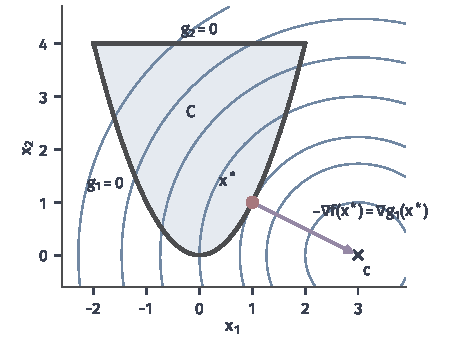
\includegraphics[width=76mm]{figures/05-optimization/06-constrained-optimization/matplotlib/nlipm-running/figure.pdf}
  \caption{贯穿例~\eqref{eq:nlipm-running}。浅蓝区域是可行集$\bm{C}$，深灰粗线是两段边界，蓝线是目标的等值线（以黑叉$\bm{c}=(3,0)$为圆心的圆），红点是最优解$\bm{x}^\star=(1,1)$。紫色箭头同时是$-\nabla f(\bm{x}^\star)$和$\nabla g_1(\bm{x}^\star)$，两者相等对应乘子$\lambda_1^\star=1$；直线边界不活动，乘子为零。}
  \label{fig:nlipm-running}
\end{BookInlineFigure}

\paragraph{内部只对不等式而言}
障碍只能加给不等式，因为只有不等式才有“里面”。记严格可行点的集合为
\begin{equation}
 \bm{C}^{\circ}=\bigl\{\bm{x}:g_i(\bm{x})<0\ (i=1,\ldots,m),\ \bm{h}(\bm{x})=\bm{0}\bigr\}.
 \label{eq:nlipm-strict-set}
\end{equation}
等式约束的可行点构成一张薄片，薄片上没有“离边界远一点”的余地。把$h=0$拆成$h\leq0$和$-h\leq0$也行不通，这两条不等式不可能同时严格成立，拆完之后$\bm{C}^{\circ}$是空集。所以等式约束继续显式保留，加上障碍之后的问题仍然是约束问题，而不是无约束问题。

\subsection{对数障碍}
\label{sec:nlipm-log-barrier}

第~\ref{chap:lp-interior-point}章对$x_i\geq0$用的障碍是$-\log x_i$。约束$x_i\geq0$也可以写成$g_i(\bm{x})=-x_i\leq0$，于是$-\log x_i=-\log(-g_i(\bm{x}))$。这个写法可以直接推广到任何$g_i$。

\begin{definition}[对数障碍函数]
\label{def:nlipm-barrier}
设$\bm{C}^{\circ}$非空。对$\mu>0$，$\bm{g}(\bm{x})<\bm{0}$的点上定义
\begin{equation}
 \phi(\bm{x})=-\sum_{i=1}^m\log\bigl(-g_i(\bm{x})\bigr),\qquad
 B_\mu(\bm{x})=f(\bm{x})+\mu\,\phi(\bm{x}).
 \label{eq:nlipm-barrier-function}
\end{equation}
相应的\term{障碍子问题}（barrier subproblem）是
\begin{equation}
 \min_{\bm{x}}\ B_\mu(\bm{x})\quad\text{s.t.}\quad\bm{h}(\bm{x})=\bm{0},\quad\bm{g}(\bm{x})<\bm{0}.
 \label{eq:nlipm-barrier-problem}
\end{equation}
\end{definition}

点靠近某条约束的边界时，$-g_i\downarrow0$，$\phi\to+\infty$。边界像一堵墙，迭代点靠函数值的上升留在内部。例~\eqref{eq:nlipm-running}的障碍目标是
\[
 B_\mu(\bm{x})=\tfrac12\bigl((x_1-3)^2+x_2^2\bigr)-\mu\log(x_2-x_1^2)-\mu\log(4-x_2).
\]
图~\ref{fig:nlipm-barrier-bowls}画出两个参数下的等值线。参数较大时碗底靠近区域中央，参数较小时等值线贴向边界，碗底被目标拉向$\bm{x}^\star$。

\begin{BookInlineFigure}
  \centering
  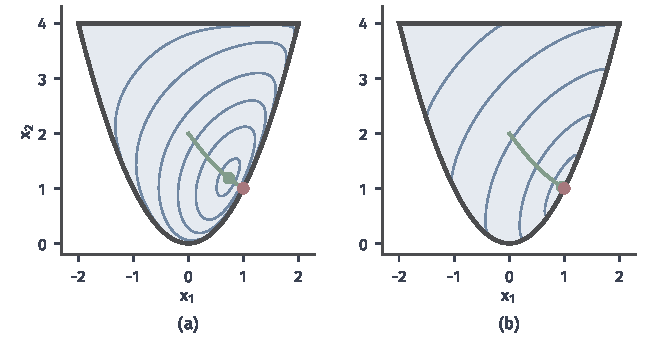
\includegraphics[width=112mm]{figures/05-optimization/06-constrained-optimization/matplotlib/nlipm-barrier-bowls/figure.pdf}
  \caption{贯穿例的障碍目标$B_\mu$在可行集内的等值线（蓝线）。(a)$\mu=1$；(b)$\mu=0.1$。绿线是各参数下碗底连成的曲线，绿点是当前参数的碗底，红点是$\bm{x}^\star$。}
  \label{fig:nlipm-barrier-bowls}
\end{BookInlineFigure}

\paragraph{约束的梯度和Hessian怎样进入}
求导只需要复合函数法则。对一元函数$\psi(u)=-\log(-u)$（$u<0$），有
\[
 \psi'(u)=\frac{1}{-u},\qquad\psi''(u)=\frac{1}{u^2}.
\]
把$u=g_i(\bm{x})$代入，并对$i$求和，得到障碍函数的梯度和Hessian：
\begin{align}
 \nabla\phi(\bm{x})&=\sum_{i=1}^m\frac{1}{-g_i(\bm{x})}\,\nabla g_i(\bm{x}),
 \label{eq:nlipm-barrier-grad}\\
 \nabla^2\phi(\bm{x})&=\sum_{i=1}^m\frac{\nabla g_i(\bm{x})\nabla g_i(\bm{x})^\top}{g_i(\bm{x})^2}
 +\sum_{i=1}^m\frac{\nabla^2g_i(\bm{x})}{-g_i(\bm{x})}.
 \label{eq:nlipm-barrier-hess}
\end{align}

式~\eqref{eq:nlipm-barrier-hess}的两项作用不同。第一项是秩一矩阵之和，只在约束的法向产生曲率，点越靠近边界越大，这就是“墙”的刚度。第二项把约束本身的弯曲带进来，线性规划中$\nabla^2g_i=\bm{0}$，这一项不存在，所以它正是本章新增的内容。

在贯穿例的点$\bm{x}=(1,2)^\top$上算一次。约束值与约束梯度是
\[
 g_1=-1,\quad g_2=-2,\quad\nabla g_1=\begin{bmatrix}2\\-1\end{bmatrix},\quad\nabla g_2=\begin{bmatrix}0\\1\end{bmatrix},\quad\nabla^2g_1=\begin{bmatrix}2&0\\0&0\end{bmatrix}.
\]
代入式~\eqref{eq:nlipm-barrier-grad}，得到
\[
 \nabla\phi=1\cdot\begin{bmatrix}2\\-1\end{bmatrix}+\frac12\begin{bmatrix}0\\1\end{bmatrix}=\begin{bmatrix}2\\-1/2\end{bmatrix}.
\]
代入式~\eqref{eq:nlipm-barrier-hess}，三块矩阵相加：
\[
 \nabla^2\phi=\begin{bmatrix}4&-2\\-2&1\end{bmatrix}+\begin{bmatrix}0&0\\0&1/4\end{bmatrix}+\begin{bmatrix}2&0\\0&0\end{bmatrix}=\begin{bmatrix}6&-2\\-2&5/4\end{bmatrix}.
\]
最后一块$\operatorname{diag}(2,0)$来自抛物线的弯曲，如果把$g_1$换成切线，它就消失了。

\paragraph{一维边界例子：内点步受到的限制}
Newton法用二次模型近似$B_\mu$，而障碍函数在边界附近根本不像二次函数。看最简单的弯约束：
\[
 \min_x\ x\quad\text{s.t.}\quad x^2-1\leq0.
\]
解是$x^\star=-1$。障碍目标$B_\mu(x)=x-\mu\log(1-x^2)$的导数是
\[
 B_\mu'(x)=1+\frac{2\mu x}{1-x^2},\qquad B_\mu''(x)=\frac{2\mu(1+x^2)}{(1-x^2)^2}.
\]
令$B_\mu'(x)=0$，得到$1-x^2+2\mu x=0$。在$(-1,1)$内的根是
\begin{equation}
 x(\mu)=\mu-\sqrt{\mu^2+1}.
 \label{eq:nlipm-1d-center}
\end{equation}
取几个能算成分数的值：$\mu=3/4$时$x=-1/2$，$\mu=5/12$时$x=-2/3$。

现在站在$\mu=3/4$的碗底$x=-1/2$，把参数减小到$\mu^+$，走一个Newton步。在这一点上
\[
 \frac{2x}{1-x^2}=-\frac43,\qquad\frac{2(1+x^2)}{(1-x^2)^2}=\frac{40}{9}.
\]
于是Newton步是
\[
 d=-\frac{1-\tfrac43\mu^+}{\tfrac{40}{9}\mu^+}=-\frac{9-12\mu^+}{40\mu^+}.
\]

$\mu^+=5/12$时$d=-6/25$，新点$-0.74$仍在区间内，离新的碗底$-2/3$不远。$\mu^+=0.05$时$d=-4.2$，新点是$-4.7$，已经远在可行域之外，如图~\ref{fig:nlipm-barrier-1d}(b)所示。要让单位步留在区间内，需要$d>-1/2$，解这个不等式，得到
\[
 \mu^+>\frac{9}{32}.
\]
也就是说，这一点上参数最多缩小到原来的$3/8$。参数一次减得太多，碗底搬走了，二次模型却还停留在旧的位置。

\begin{BookInlineFigure}
  \centering
  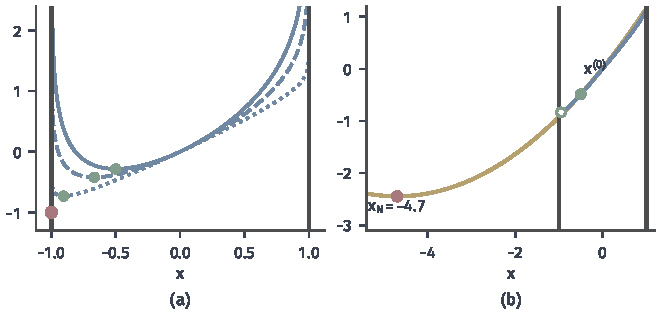
\includegraphics[width=112mm]{figures/05-optimization/06-constrained-optimization/matplotlib/nlipm-barrier-1d/figure.pdf}
  \caption{一维边界例子$\min x$，$x^2\leq1$。(a)蓝线是$B_\mu$，实线、虚线、点线分别对应$\mu=3/4$、$5/12$、$0.1$，绿点是碗底，红点是解$x^\star=-1$，深灰粗线是边界$x=\pm1$。(b)参数减到$\mu^+=0.05$，蓝线是$B_{\mu^+}$，只在区间内有定义；黄线是在绿点$x^{(0)}=-1/2$处的二次模型，其极小点（红点）落在$-4.7$；空心绿点是新的碗底。}
  \label{fig:nlipm-barrier-1d}
\end{BookInlineFigure}

\paragraph{新的曲率与凸性}
约束的弯曲方向决定第二项的符号。$g_i$凸时$\nabla^2g_i\succeq\bm{0}$，第二项半正定，障碍函数保持凸性。

\begin{lemma}[凸约束的障碍是凸函数]
\label{lem:nlipm-barrier-convex}
设每个$g_i$在开集上凸且二阶连续可微，则$\phi$在集合$\{\bm{x}:\bm{g}(\bm{x})<\bm{0}\}$的每个凸子集上是凸函数。
\end{lemma}

\begin{proof}
式~\eqref{eq:nlipm-barrier-hess}中，第一项是半正定矩阵的非负组合。第二项中$-g_i>0$，$\nabla^2g_i\succeq\bm{0}$，也是半正定矩阵的非负组合。所以$\nabla^2\phi\succeq\bm{0}$。
\end{proof}

$g_i$非凸时，这个结论没有理由成立，用了对数也不会自动得到凸子问题。看单位圆盘的外部，约束是$g(\bm{x})=1-\lVert\bm{x}\rVert_2^2\leq0$。这时$\nabla^2g=-2\bm{I}$，式~\eqref{eq:nlipm-barrier-hess}给出
\[
 \nabla^2\phi(\bm{x})=\frac{4\bm{x}\bm{x}^\top}{(\lVert\bm{x}\rVert_2^2-1)^2}-\frac{2\bm{I}}{\lVert\bm{x}\rVert_2^2-1}.
\]
沿与$\bm{x}$垂直的切向，第一项为零，第二项是负的，曲率等于$-2/(\lVert\bm{x}\rVert_2^2-1)$，离边界越近越负。

图~\ref{fig:nlipm-nonconvex-barrier}取目标$x_2^2+0.12(x_1-1/2)^2$，并取$\mu=0.1$。障碍目标有两个彼此隔开的局部极小点，分别在圆盘的右侧和左侧。图(b)沿点$(1.5,0)$处的切向对比两种约束：外部约束的障碍在这一点是山顶形状，圆盘内部约束的障碍则是碗。

\begin{BookInlineFigure}
  \centering
  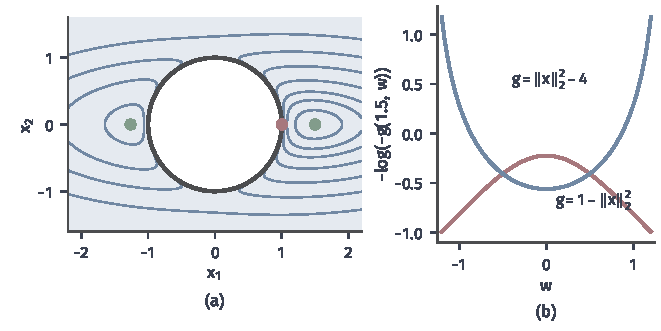
\includegraphics[width=112mm]{figures/05-optimization/06-constrained-optimization/matplotlib/nlipm-nonconvex-barrier/figure.pdf}
  \caption{非凸约束的障碍。(a)可行集是单位圆盘的外部（浅蓝），蓝线是$B_{0.1}$的等值线，两个绿点是障碍目标的局部极小点，红点是原问题的全局解$(1,0)$。(b)沿$x_1=1.5$的切向，红线是外部约束$g=1-\lVert\bm{x}\rVert_2^2$的障碍，在$w=0$处曲率为负；蓝线是圆盘内部约束$g=\lVert\bm{x}\rVert_2^2-4$的障碍，曲率为正。}
  \label{fig:nlipm-nonconvex-barrier}
\end{BookInlineFigure}

\subsection{参数与路径}
\label{sec:nlipm-parameter-path}

固定一个$\mu$，子问题~\eqref{eq:nlipm-barrier-problem}有没有解？解随$\mu$怎样变？这一小节先用驻定条件把子问题和KKT条件联系起来，再分凸问题和非凸问题回答这两个问题。

\paragraph{驻定条件就是扰动的互补}
子问题~\eqref{eq:nlipm-barrier-problem}的一阶条件是：存在$\bm{\nu}$，使
\[
 \nabla B_\mu(\bm{x})+\bm{A}(\bm{x})^\top\bm{\nu}=\bm{0}.
\]
把式~\eqref{eq:nlipm-barrier-grad}代入，得到
\[
 \nabla f(\bm{x})+\sum_{i=1}^m\frac{\mu}{-g_i(\bm{x})}\nabla g_i(\bm{x})+\bm{A}(\bm{x})^\top\bm{\nu}=\bm{0}.
\]

求和中的系数都是正数，并且正好处在KKT条件中乘子的位置。令$\lambda_i=\mu/(-g_i(\bm{x}))$，条件变成
\begin{equation}
 \begin{gathered}
 \nabla f(\bm{x})+\bm{J}(\bm{x})^\top\bm{\lambda}+\bm{A}(\bm{x})^\top\bm{\nu}=\bm{0},\qquad\bm{h}(\bm{x})=\bm{0},\\
 \lambda_i\bigl(-g_i(\bm{x})\bigr)=\mu\ (i=1,\ldots,m),\qquad\bm{g}(\bm{x})<\bm{0},\quad\bm{\lambda}>\bm{0}.
 \end{gathered}
 \label{eq:nlipm-perturbed-kkt}
\end{equation}
与KKT条件逐项比较，只有互补一处不同：$\lambda_ig_i=0$换成了$\lambda_i(-g_i)=\mu$。这和第~\ref{chap:lp-interior-point}章的$x_is_i=\mu$是同一件事。乘子不是另外猜出来的，它就是障碍项在该约束上施加的推力，$\lambda_i=\mu/(-g_i)$离墙越近越大。

\paragraph{子问题的解何时存在}
碗底的存在要靠水平集被围住。下面的定理说明，可行集有界时墙就足够了。

\begin{theorem}[障碍子问题的解]
\label{thm:nlipm-barrier-exists}
设$f$、$g_i$、$h_j$连续，可行集$\bm{C}$有界，$\bm{C}^{\circ}$非空，$\mu>0$。则$B_\mu$在$\bm{C}^{\circ}$上取到最小值。

再设$f$、$g_i$凸且二阶连续可微，$\bm{h}(\bm{x})=\bm{A}\bm{x}-\bm{b}$，$\bm{A}$满行秩，并且不存在非零的$\bm{d}$同时满足
\begin{equation}
 \bm{A}\bm{d}=\bm{0},\quad\bm{d}^\top\nabla^2f\bm{d}=0,\quad\nabla g_i^\top\bm{d}=0,\quad\bm{d}^\top\nabla^2g_i\bm{d}=0\ (\forall i)
 \label{eq:nlipm-unique-condition}
\end{equation}
（各导数在$\bm{C}^{\circ}$的任一点取值）。则最小点$\bm{x}(\mu)$唯一，方程组~\eqref{eq:nlipm-perturbed-kkt}有唯一解$(\bm{x}(\mu),\bm{\lambda}(\mu),\bm{\nu}(\mu))$。
\end{theorem}

\begin{proof}
先证存在。$\bm{C}$是有界闭集，$f$和每个$-g_i$在其上连续，所以存在常数$F$和$G>1$，使$\lvert f\rvert\leq F$，$-g_i\leq G$。

取$\bm{x}^{(0)}\in\bm{C}^{\circ}$，考虑下水平集
\[
 \bigl\{\bm{x}\in\bm{C}^{\circ}:B_\mu(\bm{x})\leq B_\mu(\bm{x}^{(0)})\bigr\}.
\]
对其中的点和任一下标$i$，把其余各项移到右边，得到
\[
 -\mu\log\bigl(-g_i(\bm{x})\bigr)\leq B_\mu(\bm{x}^{(0)})+F+\mu(m-1)\log G.
\]
右端是常数，所以存在$\epsilon>0$，使$-g_i(\bm{x})\geq\epsilon$。这说明水平集是$\bm{C}$的闭子集，从而是紧集，连续函数$B_\mu$在其上取到最小值。

再证唯一。由引理~\ref{lem:nlipm-barrier-convex}，$B_\mu$凸。对满足$\bm{A}\bm{d}=\bm{0}$的非零$\bm{d}$，式~\eqref{eq:nlipm-barrier-hess}给出
\[
 \bm{d}^\top\nabla^2B_\mu\bm{d}=\bm{d}^\top\nabla^2f\bm{d}+\mu\sum_{i=1}^m\Bigl(\frac{(\nabla g_i^\top\bm{d})^2}{g_i^2}+\frac{\bm{d}^\top\nabla^2g_i\bm{d}}{-g_i}\Bigr).
\]
右端各项非负，由条件~\eqref{eq:nlipm-unique-condition}，它们不全为零，所以$B_\mu$在仿射集上严格凸，最小点唯一。

最后看方程组。最小点处梯度与$\bm{A}$的零空间正交，所以存在$\bm{\nu}$使驻定条件成立，$\bm{A}$满行秩使$\bm{\nu}$唯一，$\bm{\lambda}$由$\lambda_i=\mu/(-g_i)$确定。反过来，方程组的解满足凸函数$B_\mu$在仿射集上的一阶条件，因此就是最小点。
\end{proof}

存在性的第一部分没有用到凸性，它只用到有界和连续。可行集无界时，这个结论可能失败。问题$\min 0$、$-x\leq0$的最优解集是$[0,\infty)$，障碍目标$-\mu\log x$在$x\to\infty$时趋于$-\infty$，没有最小点。条件~\eqref{eq:nlipm-unique-condition}在贯穿例中成立，因为$\nabla^2f=\bm{I}$，第二项已经排除了所有非零方向。

\paragraph{路径}
定理的条件成立时，$\mu$取遍$(0,\infty)$，解连成一条曲线，沿用第~\ref{chap:lp-interior-point}章的名字，称为中心路径。图~\ref{fig:nlipm-central-path}画出贯穿例的路径。当$\mu\to\infty$时，目标的作用可以忽略，点趋于$\phi$的最小点，即解析中心。贯穿例的解析中心可以直接求：对称性给出$x_1=0$，再由$-1/x_2+1/(4-x_2)=0$得到$x_2=2$。

\begin{BookInlineFigure}
  \centering
  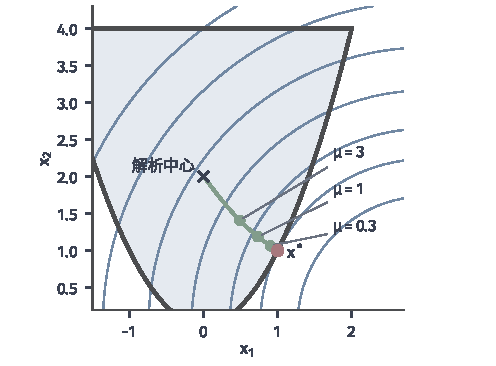
\includegraphics[width=84mm]{figures/05-optimization/06-constrained-optimization/matplotlib/nlipm-central-path/figure.pdf}
  \caption{贯穿例的中心路径（绿线）。黑叉是解析中心$(0,2)$，绿点是$\mu=3$、$1$、$0.3$对应的中心点，红点是$\bm{x}^\star=(1,1)$，蓝线是目标的等值线。路径是弯的，因为不活动的直线约束的影响在逐渐消失。}
  \label{fig:nlipm-central-path}
\end{BookInlineFigure}

这个例子的路径可以化成一元方程。由方程组~\eqref{eq:nlipm-perturbed-kkt}的第一行，$\lambda_1=(3-x_1)/(2x_1)$。取$\mu=1$，用Newton法解出的中心点和乘子是
\[
 \bm{x}(1)\approx(0.7343,1.1873)^\top,\qquad\bm{\lambda}(1)\approx(1.5428,0.3555)^\top.
\]
可以核对互补：$\lambda_1(x_2-x_1^2)=1.5428\times0.6481\approx1$，$\lambda_2(4-x_2)=0.3555\times2.8127\approx1$。

图~\ref{fig:nlipm-path-multipliers}(a)显示乘子沿路径的走向。活动约束的乘子$\lambda_1(\mu)$趋于$\lambda_1^\star=1$，不活动约束的乘子$\lambda_2(\mu)$按$\mu/3$的量级趋于零，这里的$3$就是直线约束在解处的松弛。乘子估计本身就在告诉我们哪条约束活动，这一点不需要事先猜测。

\paragraph{凸问题的间隙}
第~\ref{chap:lp-interior-point}章中，沿路径的对偶间隙恰好是$n\mu$。一般凸问题也有同样的结果，只是$n$要换成不等式的条数$m$。

\begin{theorem}[路径上的间隙]
\label{thm:nlipm-gap}
设$f$、$g_i$凸且可微，$\bm{h}(\bm{x})=\bm{A}\bm{x}-\bm{b}$，$(\bm{x},\bm{\lambda},\bm{\nu})$满足方程组~\eqref{eq:nlipm-perturbed-kkt}，$f^\star$是问题~\eqref{eq:nlipm-problem}在可行集上的下确界。则
\begin{equation}
 f(\bm{x})-m\mu\leq f^\star\leq f(\bm{x}).
 \label{eq:nlipm-gap}
\end{equation}
\end{theorem}

\begin{proof}
右边的不等式成立是因为$\bm{x}$可行。对左边，任取可行点$\bm{x}'$。因为$\bm{\lambda}>\bm{0}$、$\bm{g}(\bm{x}')\leq\bm{0}$、$\bm{h}(\bm{x}')=\bm{0}$，有
\[
 f(\bm{x}')\geq f(\bm{x}')+\bm{\lambda}^\top\bm{g}(\bm{x}')+\bm{\nu}^\top\bm{h}(\bm{x}')=\mathcal{L}(\bm{x}',\bm{\lambda},\bm{\nu}).
\]

$\mathcal{L}(\cdot,\bm{\lambda},\bm{\nu})$是凸函数，并且在$\bm{x}$处梯度为零，所以$\bm{x}$是它的全局最小点：
\[
 \mathcal{L}(\bm{x}',\bm{\lambda},\bm{\nu})\geq\mathcal{L}(\bm{x},\bm{\lambda},\bm{\nu}).
\]

再用$\bm{h}(\bm{x})=\bm{0}$和$\lambda_ig_i(\bm{x})=-\mu$，得到
\[
 \mathcal{L}(\bm{x},\bm{\lambda},\bm{\nu})=f(\bm{x})+\sum_{i=1}^m\lambda_ig_i(\bm{x})=f(\bm{x})-m\mu.
\]
三式相连，对$\bm{x}'$取下确界即得。
\end{proof}

式~\eqref{eq:nlipm-gap}的左端是一个对偶值，它由当前点直接算出，不需要知道$\bm{x}^\star$。要保证目标误差不超过$\varepsilon$，走到$\mu\leq\varepsilon/m$就够了。

这个界数的是全部$m$条约束，实际误差往往更小。图~\ref{fig:nlipm-path-multipliers}(b)中，贯穿例的$f(\bm{x}(\mu))-f^\star$在$\mu$小时约等于$\mu$，而不是$2\mu$。原因是不活动的约束虽然也贡献了$\lambda_2s_2=\mu$，它却只是把对偶值往下拉，并不代表目标还有这么多可以下降。

\begin{BookInlineFigure}
  \centering
  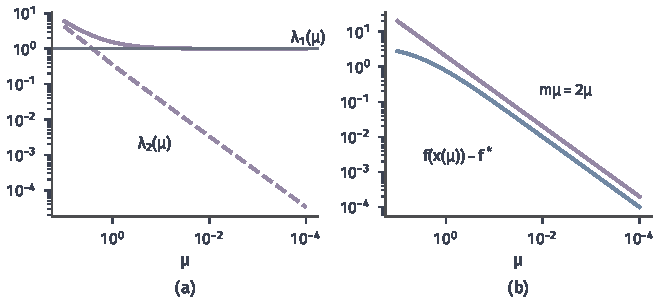
\includegraphics[width=112mm]{figures/05-optimization/06-constrained-optimization/matplotlib/nlipm-path-multipliers/figure.pdf}
  \caption{贯穿例沿中心路径的量，横轴是$\mu$，向右减小。(a)紫色实线是$\lambda_1(\mu)$，趋于$\lambda_1^\star=1$（灰线）；紫色虚线是$\lambda_2(\mu)$，随$\mu$线性趋于零。(b)紫线是定理的界$m\mu=2\mu$，蓝线是实际误差$f(\bm{x}(\mu))-f^\star$。}
  \label{fig:nlipm-path-multipliers}
\end{BookInlineFigure}

\paragraph{固定参数时解多准，参数降多快}
这样就得到\term{障碍法}（barrier method）：外层维护参数$\mu$，内层从上一个点出发，用第~\ref{chap:second-order-methods}章的阻尼Newton法解子问题~\eqref{eq:nlipm-barrier-problem}，解到Newton减量足够小，再令$\mu\leftarrow\tau\mu$，其中$\tau\in(0,1)$。回溯时要多加一条规则，试探点若使某个$g_i\geq0$，直接拒绝。

以贯穿例从$\bm{x}^{(0)}=(1,2)^\top$、$\mu=1$开始。前面已经算出$\nabla\phi$和$\nabla^2\phi$，把目标的导数加上，得到
\[
 \nabla B_1=\begin{bmatrix}0\\3/2\end{bmatrix},\qquad\nabla^2B_1=\begin{bmatrix}7&-2\\-2&9/4\end{bmatrix}.
\]
解线性方程组，Newton方向是
\[
 \bm{d}=\Bigl(-\frac{12}{47},\,-\frac{42}{47}\Bigr)^\top\approx(-0.2553,\,-0.8936)^\top.
\]
单位步后的点$(0.7447,1.1064)^\top$仍然严格可行，再走两步就到达$\bm{x}(1)$附近。

外层有两种取舍。$\tau$接近$1$时，上一个点几乎就是新碗底，每轮只需一两个Newton步，但要走很多轮。$\tau$很小时，轮数少，但正如一维例子所示，起步时Newton步很不可靠，每轮要靠回溯慢慢走。

图~\ref{fig:nlipm-update-tradeoff}是贯穿例上的实测，从解析中心出发，要求$m\mu\leq10^{-6}$。$\tau=0.9$时总共要$218$个Newton步，$\tau=0.5$时$38$步，$\tau=0.1$时$32$步，$\tau=0.001$时只要$18$步，单轮最多也不过$6$步。这说明Newton步的总数对$\tau$不敏感，只有$\tau$过于接近$1$时明显吃亏。

这是一个二维小例子上的观察，并且总数随$\tau$并不单调。规模增大时，大幅度减小参数的代价一般会更明显，第~\ref{sec:nlipm-guarantees}节再谈理论上的界。

\begin{BookInlineFigure}
  \centering
  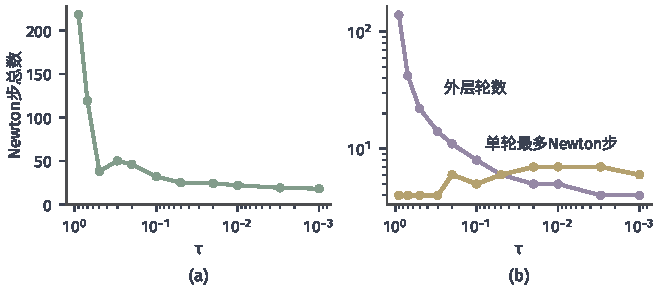
\includegraphics[width=112mm]{figures/05-optimization/06-constrained-optimization/matplotlib/nlipm-update-tradeoff/figure.pdf}
  \caption{贯穿例上障碍法的工作量，$\mu^{(0)}=1$，内层Newton减量阈值$10^{-8}$，横轴是参数缩小倍率$\tau$，向右更激进。(a)Newton步总数。(b)紫线是外层轮数，黄线是单轮最多的Newton步数。}
  \label{fig:nlipm-update-tradeoff}
\end{BookInlineFigure}

\paragraph{非凸问题只能谈局部路径}
没有凸性时，定理~\ref{thm:nlipm-gap}的推理在“$\bm{x}$是$\mathcal{L}$的全局最小点”这一步断掉，方程组~\eqref{eq:nlipm-perturbed-kkt}的解也不必唯一。能保证的是在一个性质好的KKT点附近，有一段路径通向它。

\begin{theorem}[KKT点附近的路径]
\label{thm:nlipm-local-path}
设$f$、$g_i$、$h_j$二阶连续可微，$(\bm{x}^\star,\bm{\lambda}^\star,\bm{\nu}^\star)$是KKT点，并满足三个条件：活动约束梯度与全部等式约束梯度线性无关；严格互补，即活动约束的乘子都为正；在临界方向上有
\begin{equation}
 \bm{d}^\top\nabla_{\bm{x}\bm{x}}^2\mathcal{L}(\bm{x}^\star,\bm{\lambda}^\star,\bm{\nu}^\star)\bm{d}>0,
 \label{eq:nlipm-sosc}
\end{equation}
这里临界方向指满足$\bm{A}\bm{d}=\bm{0}$、对活动约束$\nabla g_i^\top\bm{d}=0$的非零$\bm{d}$。则存在$\bar{\mu}>0$和连续可微的曲线$\mu\mapsto(\bm{x}(\mu),\bm{\lambda}(\mu),\bm{\nu}(\mu))$，在$(0,\bar{\mu})$上满足方程组~\eqref{eq:nlipm-perturbed-kkt}，$\mu\downarrow0$时趋于该KKT点，并且$\bm{x}(\mu)$是子问题~\eqref{eq:nlipm-barrier-problem}的严格局部极小点。
\end{theorem}

\begin{proof}
设$\bm{s}=-\bm{g}$，把方程组写成关于$(\bm{x},\bm{s},\bm{\lambda},\bm{\nu})$的方程$\bm{F}(\cdot)=\mu\bm{e}$，其中$\bm{e}$只在互补方程处为$1$。在$\mu=0$的KKT点处用隐函数定理，只需证明Jacobian矩阵非奇异，也就是下面的齐次方程只有零解：
\[
 \begin{gathered}
 \bm{W}\bm{d}+\bm{J}^\top\bm{d}_\lambda+\bm{A}^\top\bm{d}_\nu=\bm{0},\qquad\bm{A}\bm{d}=\bm{0},\\
 \bm{J}\bm{d}+\bm{d}_s=\bm{0},\qquad\lambda_i^\star d_{s,i}+s_i^\star d_{\lambda,i}=0.
 \end{gathered}
\]
这里$\bm{W}=\nabla^2_{\bm{x}\bm{x}}\mathcal{L}$。

对活动约束，$s_i^\star=0$、$\lambda_i^\star>0$，互补方程给出$d_{s,i}=0$，于是$\nabla g_i^\top\bm{d}=0$。对不活动约束，$\lambda_i^\star=0$、$s_i^\star>0$，互补方程给出$d_{\lambda,i}=0$。

用$\bm{d}^\top$左乘第一个方程，再用$\bm{A}\bm{d}=\bm{0}$，得到
\[
 \bm{d}^\top\bm{W}\bm{d}=-\sum_{i}d_{\lambda,i}\nabla g_i^\top\bm{d}=0.
\]
求和中每一项都为零：活动约束的$\nabla g_i^\top\bm{d}=0$，不活动约束的$d_{\lambda,i}=0$。由条件~\eqref{eq:nlipm-sosc}，$\bm{d}=\bm{0}$。

于是$\bm{d}_s=\bm{0}$，第一个方程只剩活动约束与等式约束的梯度组合等于零，由线性无关性，$\bm{d}_\lambda$、$\bm{d}_\nu$为零。隐函数定理给出连续可微的解曲线。对小的$\mu>0$，活动约束$s_i=\mu/\lambda_i>0$，不活动约束$\lambda_i=\mu/s_i>0$，所以解满足正性要求。

最后证局部极小。把式~\eqref{eq:nlipm-barrier-hess}和$\lambda_i=\mu/s_i$代入$\nabla^2B_\mu$，并计入等式约束的曲率，子问题的Lagrange Hessian是$\bm{W}+\bm{J}^\top\bm{S}^{-1}\bm{\Lambda}\bm{J}$，其中$\bm{S}$、$\bm{\Lambda}$是对角矩阵。假设存在$\mu_k\downarrow0$和单位向量$\bm{d}_k$，满足$\bm{A}\bm{d}_k=\bm{0}$，而二次型非正。则
\[
 \sum_{i}\frac{\lambda_i}{s_i}(\nabla g_i^\top\bm{d}_k)^2\leq-\bm{d}_k^\top\bm{W}\bm{d}_k.
\]
右端有界，而活动约束的$\lambda_i/s_i\to\infty$，所以极限方向$\bar{\bm{d}}$满足$\nabla g_i^\top\bar{\bm{d}}=0$。于是$\bar{\bm{d}}$是临界方向，并且$\bar{\bm{d}}^\top\bm{W}\bar{\bm{d}}\leq0$，与式~\eqref{eq:nlipm-sosc}矛盾。
\end{proof}

定理的三个条件各管一件事。线性无关保证乘子唯一，严格互补保证每条约束在极限时明确属于活动或不活动的一侧，式~\eqref{eq:nlipm-sosc}保证弯曲方向上是极小而不是鞍点。

隐函数定理还给出路径在$\mu=0$处的切线。在贯穿例中，$\bm{W}=\operatorname{diag}(3,1)$，$s_2^\star=3$，把解曲线对$\mu$求导，得到
\[
 \lambda_2'(0)=\frac13,\qquad s_1'(0)=1.
\]
线性化的方程剩下三个未知量$x_1'$、$x_2'$、$\lambda_1'$，解出
\[
 \bm{x}'(0)=\Bigl(-\frac{8}{21},\,\frac{5}{21}\Bigr)^\top,\qquad\lambda_1'(0)=\frac47.
\]
所以$\bm{x}(\mu)\approx(1,1)^\top+\mu(-8/21,5/21)^\top$。取$\mu=0.01$，预测$(0.9962,1.0024)^\top$，数值解是$(0.9962,1.0024)^\top$。目标的一阶变化是$\nabla f^\top\bm{x}'(0)=1$，这正是前面看到的“误差约等于$\mu$”。

\paragraph{路径可以断开，也可能通向较差的解}
定理~\ref{thm:nlipm-local-path}的$\bar{\mu}$可以很小，它不保证路径能一直延伸到大的$\mu$。下面的一维例子说明会发生什么。在$x>0$上取$f'(x)=(x-1)(x-3)(x-4)$，它在$x=1$和$x=4$处有局部极小，$f(4)-f(1)=9/4$，所以$x=1$是全局解。

障碍驻定条件$f'(x)=\mu/x$可以反解成
\[
 \mu=x(x-1)(x-3)(x-4).
\]
要求$\mu>0$，可行的$x$只有$(1,3)$和$(4,\infty)$两段。第一段上$\mu$先增后减，在$x=2$处达到最大值$\mu=4$。图~\ref{fig:nlipm-nonconvex-fold}(b)中，极小点的分支从$x=1$出发，到$\mu=4$时与鞍点分支相撞，两者同时消失，这个点称为\term{折叠点}（fold point）。

$\mu>4$时只剩$x>4$这一支。从大的$\mu$出发沿路径减小参数，走到的是$x=4$，错过了全局解$x=1$。这条路径是连续的，算法并没有失败，只是路径根本不经过全局解。

\begin{BookInlineFigure}
  \centering
  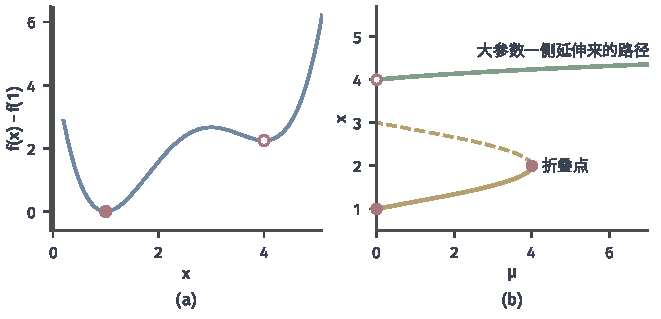
\includegraphics[width=112mm]{figures/05-optimization/06-constrained-optimization/matplotlib/nlipm-nonconvex-fold/figure.pdf}
  \caption{非凸的一维路径，$f'(x)=(x-1)(x-3)(x-4)$，$x>0$。(a)蓝线是目标，红点是全局解$x=1$，空心红点是局部解$x=4$。(b)$(\mu,x)$平面上的驻点集合：绿线是从大参数一侧延伸来的路径；黄线是$(1,3)$上的另一支，实线部分是局部极小点，虚线部分不是，两者在红点（折叠点$(4,2)$）相遇。}
  \label{fig:nlipm-nonconvex-fold}
\end{BookInlineFigure}
